%%%%%%%%%%%%%%%%%%%%%%%%%%%%%%%%%%%%%%%%%
% Article EcoFoG
% Version 2.1 (23/10/2017)
%
% adapté de :
% Stylish Article
% LaTeX Template
% Version 1.0 (31/1/13)
%
% This template has been downloaded from:
% http://www.LaTeXTemplates.com
%
% Original author:
% Mathias Legrand (legrand.mathias@gmail.com)
%
% License:
% CC BY-NC-SA 3.0 (http://creativecommons.org/licenses/by-nc-sa/3.0/)
%
%%%%%%%%%%%%%%%%%%%%%%%%%%%%%%%%%%%%%%%%%


%----------------------------------------------------------------------------------------
%	PACKAGES AND OTHER DOCUMENT CONFIGURATIONS
%----------------------------------------------------------------------------------------

\documentclass[fleqn,10pt]{ArtEcoFoG} % Document font size and equations flushed left

\setcounter{tocdepth}{3} % Show only three levels in the table of contents section: sections, subsections and subsubsections


% Pandoc environments
\usepackage{framed}
\usepackage{fancyvrb}
\providecommand{\tightlist}{%
  \setlength{\itemsep}{0pt}\setlength{\parskip}{0pt}}
\newcommand{\VerbBar}{|}
\newcommand{\VERB}{\Verb[commandchars=\\\{\}]}
\DefineVerbatimEnvironment{Highlighting}{Verbatim}{commandchars=\\\{\}, fontsize=\scriptsize} % Code R
\definecolor{shadecolor}{RGB}{248,248,248}
\newenvironment{Shaded}{\begin{snugshade}}{\end{snugshade}}
\newcommand{\KeywordTok}[1]{\textcolor[rgb]{0.13,0.29,0.53}{\textbf{{#1}}}}
\newcommand{\DataTypeTok}[1]{\textcolor[rgb]{0.13,0.29,0.53}{{#1}}}
\newcommand{\DecValTok}[1]{\textcolor[rgb]{0.00,0.00,0.81}{{#1}}}
\newcommand{\BaseNTok}[1]{\textcolor[rgb]{0.00,0.00,0.81}{{#1}}}
\newcommand{\FloatTok}[1]{\textcolor[rgb]{0.00,0.00,0.81}{{#1}}}
\newcommand{\ConstantTok}[1]{\textcolor[rgb]{0.00,0.00,0.00}{{#1}}}
\newcommand{\CharTok}[1]{\textcolor[rgb]{0.31,0.60,0.02}{{#1}}}
\newcommand{\SpecialCharTok}[1]{\textcolor[rgb]{0.00,0.00,0.00}{{#1}}}
\newcommand{\StringTok}[1]{\textcolor[rgb]{0.31,0.60,0.02}{{#1}}}
\newcommand{\VerbatimStringTok}[1]{\textcolor[rgb]{0.31,0.60,0.02}{{#1}}}
\newcommand{\SpecialStringTok}[1]{\textcolor[rgb]{0.31,0.60,0.02}{{#1}}}
\newcommand{\ImportTok}[1]{{#1}}
\newcommand{\CommentTok}[1]{\textcolor[rgb]{0.56,0.35,0.01}{\textit{{#1}}}}
\newcommand{\DocumentationTok}[1]{\textcolor[rgb]{0.56,0.35,0.01}{\textbf{\textit{{#1}}}}}
\newcommand{\AnnotationTok}[1]{\textcolor[rgb]{0.56,0.35,0.01}{\textbf{\textit{{#1}}}}}
\newcommand{\CommentVarTok}[1]{\textcolor[rgb]{0.56,0.35,0.01}{\textbf{\textit{{#1}}}}}
\newcommand{\OtherTok}[1]{\textcolor[rgb]{0.56,0.35,0.01}{{#1}}}
\newcommand{\FunctionTok}[1]{\textcolor[rgb]{0.00,0.00,0.00}{{#1}}}
\newcommand{\VariableTok}[1]{\textcolor[rgb]{0.00,0.00,0.00}{{#1}}}
\newcommand{\ControlFlowTok}[1]{\textcolor[rgb]{0.13,0.29,0.53}{\textbf{{#1}}}}
\newcommand{\OperatorTok}[1]{\textcolor[rgb]{0.81,0.36,0.00}{\textbf{{#1}}}}
\newcommand{\BuiltInTok}[1]{{#1}}
\newcommand{\ExtensionTok}[1]{{#1}}
\newcommand{\PreprocessorTok}[1]{\textcolor[rgb]{0.56,0.35,0.01}{\textit{{#1}}}}
\newcommand{\AttributeTok}[1]{\textcolor[rgb]{0.77,0.63,0.00}{{#1}}}
\newcommand{\RegionMarkerTok}[1]{{#1}}
\newcommand{\InformationTok}[1]{\textcolor[rgb]{0.56,0.35,0.01}{\textbf{\textit{{#1}}}}}
\newcommand{\WarningTok}[1]{\textcolor[rgb]{0.56,0.35,0.01}{\textbf{\textit{{#1}}}}}
\newcommand{\AlertTok}[1]{\textcolor[rgb]{0.94,0.16,0.16}{{#1}}}
\newcommand{\ErrorTok}[1]{\textcolor[rgb]{0.64,0.00,0.00}{\textbf{{#1}}}}
\newcommand{\NormalTok}[1]{{#1}}
\usepackage{longtable,booktabs}
\usepackage{caption}
% These lines are needed to make table captions work with longtable:
\makeatletter
\def\fnum@table{\tablename~\thetable}
\makeatother
% longtable 2 columns
% https://tex.stackexchange.com/questions/161431/how-to-solve-longtable-is-not-in-1-column-mode-error
\makeatletter
\let\oldlt\longtable
\let\endoldlt\endlongtable
\def\longtable{\@ifnextchar[\longtable@i \longtable@ii}
\def\longtable@i[#1]{\begin{figure}[t]
\onecolumn
\begin{minipage}{0.5\textwidth}\scriptsize
\oldlt[#1]
}
\def\longtable@ii{\begin{figure}[t]
\onecolumn
\begin{minipage}{0.5\textwidth}\scriptsize
\oldlt
}
\def\endlongtable{\endoldlt
\end{minipage}
\twocolumn
\end{figure}}
\makeatother

\usepackage{graphicx,grffile}
\makeatletter
\def\maxwidth{\ifdim\Gin@nat@width>\linewidth\linewidth\else\Gin@nat@width\fi}
\def\maxheight{\ifdim\Gin@nat@height>\textheight0.8\textheight\else\Gin@nat@height\fi}
\makeatother
% Scale images if necessary, so that they will not overflow the page
% margins by default, and it is still possible to overwrite the defaults
% using explicit options in \includegraphics[width, height, ...]{}
\setkeys{Gin}{width=\maxwidth,height=\maxheight,keepaspectratio}

% User-adder preamble
\usepackage{textcomp} \DeclareUnicodeCharacter{B0}{\textdegree}
\usepackage{tabu}
\renewenvironment{table}{\begin{table*}}{\end{table*}\ignorespacesafterend}
\hyphenation{bio-di-ver-si-ty sap-lings post-dis-tur-bance}
\hypersetup{draft}

%----------------------------------------------------------------------------------------
%	ARTICLE INFORMATION
%----------------------------------------------------------------------------------------

\JournalInfo{Hal xxx} % Journal information
\Archive{DOI xxxx} % Additional notes (e.g. copyright, DOI, review/research article)

\PaperTitle{30 Years of Post-disturbance Recruitment in Tropical Forest} % Article title

\Authors{
Ariane MIRABEL\textsuperscript{1*}\\ Eric MARCON\textsuperscript{1}\\ Bruno HERAULT\textsuperscript{2}
} % Authors
\affiliation{
\textsuperscript{1}UMR EcoFoG, AgroParistech, CNRS, Cirad, INRA, Université des Antilles,
Université de Guyane.\\ \hspace{1em} Campus Agronomique, 97310 Kourou, France.\\\textsuperscript{2}INPHB (Institut National Ploytechnique Félix Houphoüet Boigny)\\ \hspace{1em} Yamoussoukro, Ivory Coast
}
\affiliation{*\textbf{Corresponding author}: ariane.mirabel@ecofog.gf, http://www.ecofog.gf/spip.php?article47} % Corresponding author

\Keywords{Taxonomic and Functional Diversity, Recruitment, Resilience, Tropical Forests, Disturbance Dynamics} % Keywords - if you don't want any simply remove all the text between the curly brackets
\newcommand{\keywordname}{Keywords} % Defines the keywords heading name

%----------------------------------------------------------------------------------------
%	ABSTRACT
%----------------------------------------------------------------------------------------

\Abstract{
Trees biodiversity is central for tropical forests functioning and
services. In the current climatic and land-use changing context it is
urgent to clarify the response of communities diversity and composition
to disturbance. Succession patterns shaped by deterministic recruitment
processes are recognized to shape communities trajectories after
disturbance but those need be tested for highly biodiverse tropical
forests and for cases where the initial communities are partly
maintained like selective logging and climatic changes. Recruitment
trajectories would allow (i) disentangling neutral, stochastic and
deterministic, selective processes shaping post-disturbance succession,
and (ii) clarify the taxonomic and functional facets of forests
resilience. We examined the trajectories over 30 years of recruitment
diversity and composition in 75 ha of a neotropical forest following a
gradient of logging and thinning disturbance (from 15 to 60\% of AGB
removed). Specifically we analysed and compared to neutral models the
recruitment trajectories in taxonomic richness, evennes, and
compositional turnover compared to initial communities, and in Rao
functional diversity integrating species ecology through 7 key
functional traits. We evidenced three recruitment phases shaped by the
gradual balance between stochastic and deterministic processes. First,
trajectories relied upon the growth of saplings randomly recruited among
the pre-disturbance community. Second, trajectories relied on \emph{true
recruits} germinated from the seeds bank and selected through
competitive exclusion for light favoring acquisitive, light-demandings
species. Eventually an inversed balance progressively restored the
stochastic recruitment observed in undisturbed forests. Recruitment
trajectories ensured both functional an dtaxonomic recovery, thus
maintaining communitiesinitial differences. Communities disturbance
response was driven by the emergence of deterministic competition
processes for light that balanced stochastic processes observed in
undisturbed forests. Communities taxonomic and functional
characteristics were consistently restored and initial differences among
commmunities were maintained. Still, the recovery was decades-long and
called cautions regarding the time prescribed for forest recovery.
}

%----------------------------------------------------------------------------------------

\begin{document}

\selectlanguage{english}

\flushbottom % Makes all text pages the same height

\maketitle % Print the title and abstract box

\tableofcontents % Print the contents section

\thispagestyle{empty} % Removes page numbering from the first page

%----------------------------------------------------------------------------------------
%	ARTICLE CONTENTS
%----------------------------------------------------------------------------------------


\section{Introduction}\label{introduction}

Determining the response of tropical forests to disturbance is key to
predict their fate in the global changing context. In the last decades,
tropical forests experienced a wide range of disturbance, from radical
land-use changes for agriculture or mining
\citep{Dezecache2017a, Dezecache2017b} to more insidious changes of
communities structure, diversity and functioning following climatic
changes \citep{Aubry-Kientz2015} or anthropogenic activities like
selective logging \citep{Baraloto2012a, Herault2016}. In that respect a
vast litterature successfully modeled communities response to
disturbance in terms of tree growth \citep{Gourlet-Fleury2000}, tree
height \citep{Rutishauser2016}, carbon, water and nutrient fluxes
\citep{Putz2012, Martin2015, Piponiot2016}. However, similar approaches
regarding forest diversity remain hindered by the scarcity of long-term
monitoring and by the huge biological diversity imposing to focus on
common or commercial species
\citep{Sebbenn2008, Rozendaal2010, Vinson2015}. Trees diversity is a
major determinant of forests functioning and productivity, so it is
urgent to elucidate its response to disturbance and the underlying
mechansisms. The diversity response would assess communities resilience
and recovery time, and eventually help adjusting exploitation and
conservation guidelines \citep{Diaz2005, Gardner2007, Schwartz2017}.

Communities response to intense disturbance have been recognized to
follow succession models based on changes in resources availability and
interactions among species. First, the succession patterns involves
already grown saplings that establish under conditions of high light,
high nutrient availability and low competition. A second phase sees the
tree growth increasing the competition for the space and resources until
excluding species with respect to their functional strategy and
competitive ability. Eventually a third phase corresponds to the
senescence of the first established seedlings and to the emergence of
understory species restoring the composition and diversity of
pre-disturbance communities. This succession model proved relevant in
temperate forests but might be blurried in tropical rainforests by their
biodiversity and by tree species rapid vegetative growth
\citep{Denslow2000}. Besides the succession model predicts forests
trajectories after very intense disturbance or clear cutting, but it
might not be as robust in cases of climatic changes or selecive logging
where the pre-disturbance communities and their steady-state dynamics
still remain. In those cases communities trajectories would depend on
both on the dynamics of surviving trees from before disturbance, and on
the recruitment of new trees \citep{Herault2018}. The recruitment in
tropical forests either rely upon stochastic processes driven only by
recruitment and dispersal limitations \citep{Hurtt1995, Hubbell2001}, or
upon deterministic processes driven by niche-based competition and
biotic interactions \citep{Adler2007}. Stochastic processes, translating
Hubbell's neutral theory, build communities as random samples of the
larger regional-scale forest \citep{Hubbell2001, Chave2004}. In contrast
deterministic processes select species with respect to their ecology and
competitive ability. The involvment of stochastic and deterministic
processes remains debated and post-disturbance trajectories probably
result from a gradual balance between them.

Communities are defined by their taxonomic characteristics, that refer
to a neutral species assemblages, and by their functional
characteristics, that account for species ecology and ecosystem
functioning \citep{Violle2007b, Kunstler2016}. The ecological processes
shaping recruitment trajectories may differently affect communities
taxonomic and functional characteristics, and two communities may be
very different in terms of taxonomy but very similar in terms of
functioning \citep{Villeger2012}. The correlations, or not, between
taxonomic and functional {[}??? system{]} trajectories are therefore
insightful of the ecological rules involved in the recruitment
processes, specifically to explicit the deterministic processes at stake
\citep{Mayfield2010, Fukami2005}. Competitive interactions among species
indeed depend on their functional differences, specifically regarding
the use of the limited shared resources, that determine their
competitive ability and ecological niche \citep{Webb2002, Perronne2017}.
In tropical forests where the light is limiting, communities response to
disturbance translate in a shift from slow-growing, long-lived species
with ``conservative'' resource use to fast growing, resource
``acquisitive'' species \citep{Denslow1980, Molino2001, Bongers2009}.\\
The competition processes at stake would be grasped by shifts in key
leaf, wood and life-history functional traits assessing species
resources acquisition strategy and ecology
\citep{Wright2004, Chave2009b, Herault2011, Gerhold2015}.

Beyond the mere understanding of response mechanisms, disentangle
deterministic from stochastic processes elucidates the resilience of
communities. Controversies remain about whether resilience is either
deterministic, entailing the convergence of communities towards stable
taxonomic and functional characteritics likely defined by the
environment \citep{Clements1916}, or stochastic, entailing species
stochastic recruitment and communities random divergence
\citep{Diamond1975}. These contrasting views were reconciled under the
hypothesis that communities might diverge in the taxonomic space while
they converge in the functional space. Under this hypothesis communities
have a determined diversity and composition in functional niches, but
this hypothesis remains to be tested in tropical forests.

In this paper we followed the fate of recruited tree diversity and
composition (60 121 individuals) over 30 years after a large disturbance
gradient, with 10 to 60\% of forest biomass removed. We assessed the
taxonomic dissimilarity between recruited trees and initial communities,
the taxonomic and functional diversity of recruited trees and the
corresponding trajectories of functional traits, using a large
functional trait database covering the leaf, wood and life-history
spectra. We compared the observed trajectories to neutral processes
corresponding to the stochastic recruitment of individuals and to the
randomization of species functional traits. These trajectories aimed to
highlight the recruitment processes underlying forests response to
disturbance, specifically assessing (i) the succession pattern and the
underlying ecological processes and (ii) clarify the taxonomic and
functional facets of forests resilience and their consequences for
forest management.

\section{Material and Methods}\label{material-and-methods}

\subsection{Study Site}\label{study-site}

The Paracou station is located in a lowland tropical rain forest in
French Guiana (518'N and 5253'W). Climate is tropical wet with mean
annual precipitation averaging 2980 mm.y\textsuperscript{-1} (30-y
period) and a 3-months dry season (\textless{} 100
mm.months\textsuperscript{-1}) from mid-August to mid-November, and a
one-month dry season in March \citep{Wagner2011}. Elevation ranges from
5 to 50 m and mean annual temperature is 26 C. Soils are thin acrisols
over a layer of transformed saprolite with low permeability generating
lateral drainage during heavy rains. The disturbance experiment spread
over a network of twelve 6.25ha plots (Table \ref{tab:Tab1}) that
underwent three disturbance treatments in 1986-1987 \citep{Herault2018}.
Dominant families are Fabaceae, Chrysobalanaceae, Lecythidaceae and
Sapotaceae.

\begin{table}

\caption{\label{tab:Tab1}Intervention table, summary of the disturbance intensity for the 4 plot treatments in Paracou.}
\centering
\begin{tabu} to \linewidth {>{\raggedright}X>{\raggedright}X>{\raggedright}X>{\raggedright}X>{\raggedright}X}
\toprule
Treatment & Timber & Thinning & Fuelwood & \%AGB lost\\
\midrule
Control &  &  &  & 0\\
T1 & DBH $\geq$ 50 cm, commercial species, $\approx$ 10 trees/ha &  &  & $[12\%-33\%]$\\
T2 & DBH $\geq$ 50 cm, commercial species, $\approx$ 10 trees/ha & DBH $\geq$ 40 cm, non-valuable species, $\approx$ 30 trees/ha &  & $[33\%-56\%]$\\
T3 & DBH $\geq$ 50 cm, commercial species, $\approx$ 10 trees/ha & DBH $\geq$ 50 cm, non-valuable species, $\approx$ 15 trees/ha & 40 cm $\leq$ DBH $\leq$ 50 cm, non-valuable species, $\approx$ 15 trees/ha & $[35\%-56\%]$\\
\bottomrule
\end{tabu}
\end{table}

\subsection{Inventories Protocol and Dataset
Collection}\label{inventories-protocol-and-dataset-collection}

All trees above 10 cm DBH were mapped and measured annually since 1984.
During inventories, trees were first identified with a vernacular name
assigned by the field team, and afterward with a scientific name
assigned by a botanist during regular botanical campaigns. Botanical
campaigns have been carried out every 5 to 6 years from 2003 onwards.
These changes in identification protocol raised methodological issues as
vernacular names usually correspond to different botanical species,
resulting in significant taxonomic uncertainties that had to be
propagated to composition and diversity metrics. Vernacular names were
replaced through multinomial trials
\(M_v\Big(\big[s_1, s_2, …, s_N\big],\big[\alpha_1, \alpha_2,…, \alpha_3\big]\Big)\)
based on the observed association probability
\(\big[\alpha_1, \alpha_2,…, \alpha_3\big]\) between each vernacular
name \emph{v} and the species \(\big[s_1, s_2, …, s_N\big]\) recorded in
the inventory. See appendix 1 and \citet{Aubry-Kientz2013} for the
detailed methodology. To avoid remaining identification caveats, the
simulated botanical inventories were reported at genus level.

Eight functional traits representing the leaf economic (leaves
thickness, toughness, total chlorophyll content and specific leaf area)
and wood economic spectra (wood specific gravity and bark thickness),
and life history traits (maximum specific height and seed mass) were
considered. Traits were exctracted from the BRIDGE project \footnote{http://www.ecofog.gf/Bridge/}
where trait values were measured on nine forest plots infrench guianan,
including two in Paracou. Missing trait values of the trait database
(10\%) were filled by multivariate imputation by chained equation using
the Mice R package \citep{Mice2011}. F-tests demonstrated that traits
variance were essentially lower within genera and families compared to
the whole inventory: we accounted for the phylogenetic signal of the
functional traits by restricting the gap filling processes to samples
pertaining to the next higher taxonomic level. As seed mass information
corresponded to a classification into discrete mass classes, no data
filling process was applied and analysis were performed only considering
the 414 botanical species of the seed mass dataset.

\subsection{Recruitment trajectories}\label{recruitment-trajectories}

To tease apart recruitment trajectories communities were split into
per-disturbance surviving trees and recruited trees afterward. Recruited
communities were examined either considering the ``punctual
recruitment'', \emph{i.e.} recruited trees by 2-year intervals, or all
recruits since disturbance as the ``accumulated recruits''. Eventually,
in disturbed plots the recruited communities were examined
distinguishing the undisturbed and logging gap areas to test the
validity of recruitment processes for the whole plot scale (see Annexe
I).

The taxonomic diversity was assessed through Richness and the Hill
number translation of Shannon and Simpson indices
\citep{Hill1973, chao2015estimating, Marcon2015b}.\\
The three diversities belong to the set of HCDT or generalized entropy,
respectively corresponding to the 0, 1 and 2 order of diversity
(\emph{q}), which grasps the balance between richness and evenness in
the community through the value of \emph{q} that emphasizes common
species. Functional trajectories were estimated with the Rao quadratic
entropy, summerizing the functional richness and evenness
\citep{Clark2012} through the measure of communities functional
divergence using Gower distance as recommended by \citet{Pavoine2009}.
Functional diversity was completed by the trajectories of traits
community weighted means (CWM), representing the average trait value in
a community weighted by relative abundance of the species carrying each
value \citep{Diaz2007, Garnier2004, Mason2013}. Seed mass trajectories
were reported by the proportion of each class recorded in the
inventories. The similarity between recruited trees and pre-disturbance
forest was measured with the turnover metrics detailed in
\citet{Podani2013a}. To estimate the importance of stochastic processes
the recruitment was compared to the trajectories of a stochastic model
of random samplings. For the taxonomic trajectories the stochastic model
was a random sampling of individuals among surviving trees according to
their observed abundance that preserved species abundance and tree
density. For the functional diversity the stochastic model was a random
reassignment of functional trait values among species that randomizes
abundances across species but within communities \citep{Mason2013}.

All composition and diversity metrics corresponded to the median and
90\% percentile obtained after 50 iterations of the taxonomy uncertainty
propagation and gap filling frameworks. The stochastic trajectories were
similarily obtained after 50 iterations of the random sampling.

\section{Results}\label{results}

\subsection{Recruitment Diversity}\label{recruitment-diversity}

All the trajectories were identical in disturbed and undisturbed areas,
confirming that recruitment processes applied to whole communities and
not restricted to logging gaps.

\subsubsection{Taxonomic Diversity}\label{taxonomic-diversity}

The diversity trajectories of punctual recruitment followed a consistent
trajectory after disturbance, first with an increase of the richness and
a decrease of the evenness (Figure (\ref{fig:DivTraj}). For all
disturbed plots both richness and evenness tended to return towards
initial values but none had recovered 30 years after disturbance. The
accumulated recruits displayed sharp increasing richness (order 0) and
decreasing evenness (order 2) after intense disturbance (T3 and some T2,
Appendix I, fig. S1).

\begin{figure*}

{\centering 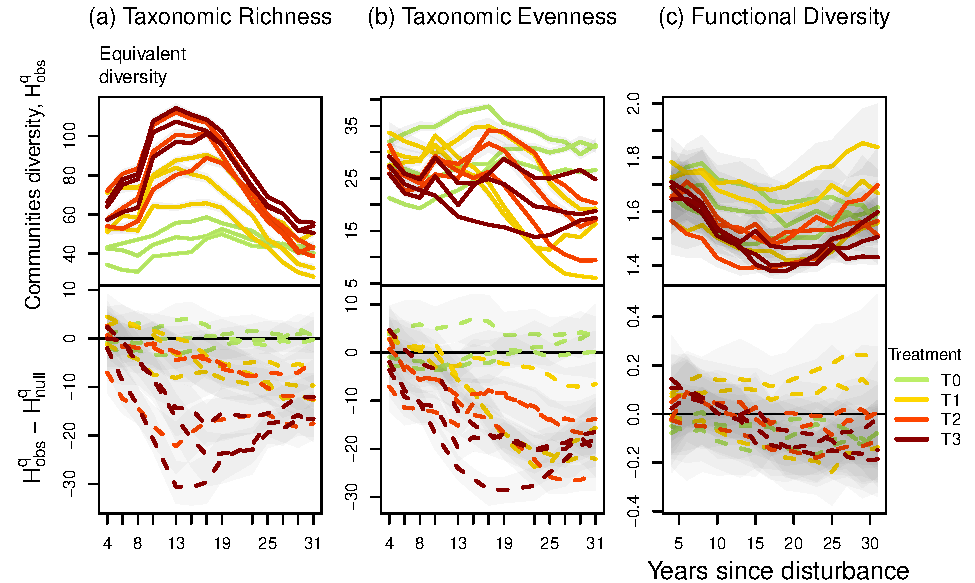
\includegraphics[width=0.8\linewidth]{RecruitmentTrajectories_files/figure-latex/DivTraj-1} 

}

\caption{Trajectories over 30 years of Richness, Shannon and Simpson diversities of punctual  recruitment (2-years laps, upper panels) and divergence to null model (lower panels). Values reported correspond to plot-level 0.025 and 0.975 percentiles (grey envelopes) and median (solid or dotted lines) obtained after 50 repetitions of the taxonomic uncertainty propagation and the functional database gap-filling frameworks. Colors correspond to the disturbance intensity (green for control, blue for T1, orange for T2 and red for T3, see Table 1 for details).}\label{fig:DivTraj}
\end{figure*}

Compared to stochastic trajectories, bserved richness (order 0) and
evenness (order 2) of punctual recruitment remained equivalent or higher
than for a random sampling in control plots while both were lower in
disturbed plots. Disturbed plots followed humped shaped trajectories
heading towards a recovery of the initial state (Figure
\ref{fig:DivTraj}). Accumulated recruitment richness and evenness were
higher or equivalent to those of a random sampling after low disturbance
intensity (plots T1 and some plots T2) but lower after intense
disturbance (plots T3 and a plot T2, Appendix I fig. S1).

\subsubsection{Functional Diversity and
Composition}\label{functional-diversity-and-composition}

In disturbed plots (T2 and T3), the functional diversity decreased until
15 years after disturbance (Figure \ref{fig:FunTraj}) before recovering
towards initial values. If the recovery was not achieved for the most
disturbed plots, it was faster after the low disturbance intensity and
for some T1 plots exceeded the initial values 30 years after
disturbance. For both disturbed and undisturbed plots, the observed
functional diversity was lower than this of the random model, to the
exception of two plots T1.

\begin{figure}

{\centering 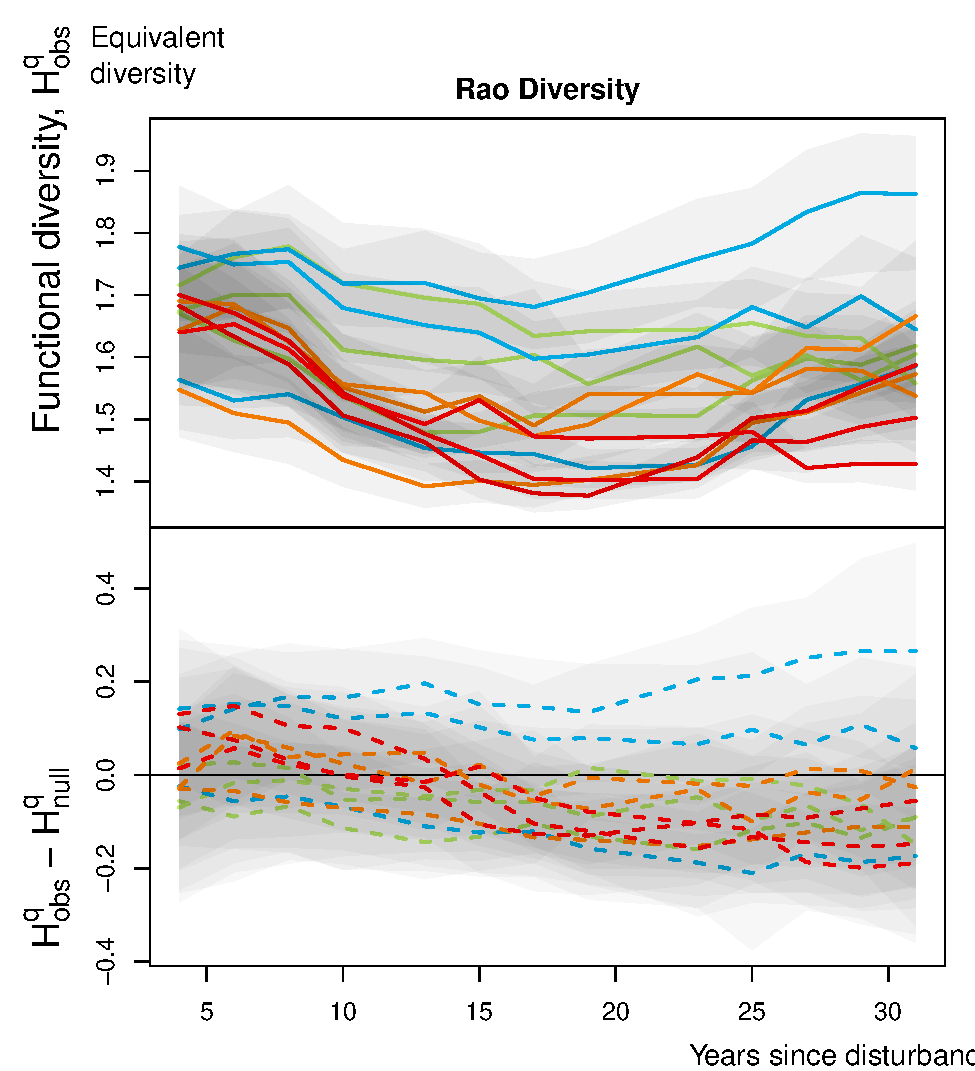
\includegraphics{RecruitmentTrajectories_files/figure-latex/FunTraj-1} 

}

\caption{Functional diversity of punctual recruited trees (2-years laps) from the 7 functional traits (upper panel) and divergence to null model (lower panel). Values reported correspond to plot-level 0.025 and 0.975 percentiles (grey envelopes) and median (solid lines) obtained after 50 run of the null model and 50 repetitions of the taxonomic uncertainty propagation and the functional database gap-filling frameworks. Colors correspond to the disturbance intensity (green for control, blue for T1, orange for T2 and red for T3, see Table 1 for details).}\label{fig:FunTraj}
\end{figure}

Trajectories of the functional traits showed a switch in disturbed plots
towards species with large exchange surface area, light tissues (high
SLA, low leaf toughness and thickness and low wood specific gravity) and
with smaller maximum height (Figure \ref{fig:CWM}). Functional traits
either followed humped shaped trajectories with an ongoing recovery or
an achieved return to the initial state (for SLA, Bark thickness and
leaf thickness and Hmax to a certain extent).

\begin{figure*}

{\centering 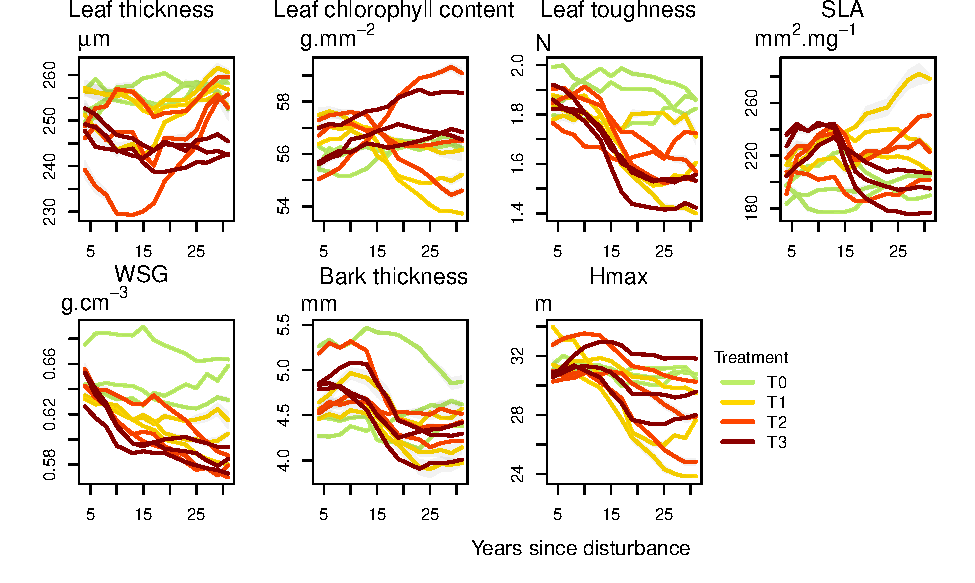
\includegraphics[width=0.8\linewidth]{RecruitmentTrajectories_files/figure-latex/CWM-1} 

}

\caption{Community weighted means (CWM) of the four leaf traits, the two stem traits and the specific maximum height. Values reported correspond to plot-level 0.025 and 0.975 percentiles (grey envelopes) and median (solid lines) obtained after 50 repetitions of the taxonomic uncertainty propagation and the functional database gap-filling frameworks. Colors correspond to the disturbance intensity (green for control, blue for T1, orange for T2 and red for T3, see Table 1 for details).}\label{fig:CWM}
\end{figure*}

\subsection{Recruitment Turnover}\label{recruitment-turnover}

In control plots species turnover remained highly stable for the 30
sampled years (Figure \ref{fig:Turnover}), reflecting a strong
similarity between the initial plots composition and the punctual
recruits. In disturbed plots, the taxonomic turnover followed a marked
humped shaped trajectory, with a maximum reached around 15 years after
disturbance and a value positively correlated to the disturbance
intensity (\(\rho_{spearman}=0.93\)). Thirty years after disturbance the
turnover of all disturbed plots had returned to low values close to
zero.

\begin{figure}

{\centering 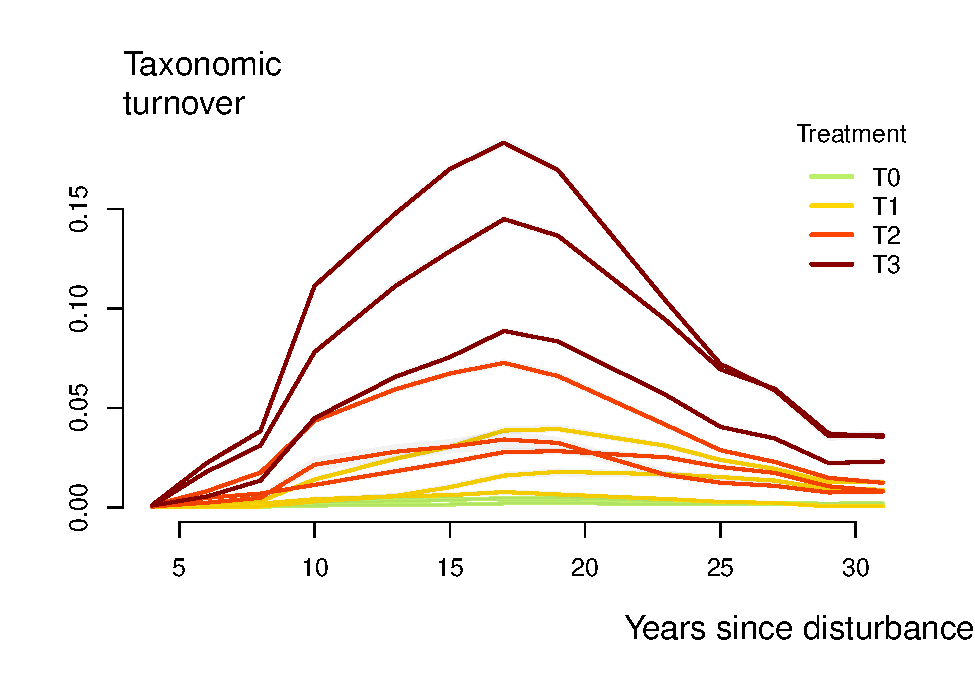
\includegraphics{RecruitmentTrajectories_files/figure-latex/Turnover-1} 

}

\caption{Trajectories over 30 years of the abundance-based turnover between recruited trees (2-years laps) and initial communities before disturbance. Values reported correspond to plot-level 0.025 and 0.975 percentiles (grey envelopes) and median (solid lines) obtained after 50 repetitions of the taxonomic uncertainty propagation framework. Colors correspond to the disturbance intensity (green for control, blue for T1, orange for T2 and red for T3, see Table 1 for details).}\label{fig:Turnover}
\end{figure}

\section{Discussion}\label{discussion}

\subsection{A three-phased succession shaped by deterministic
processes}\label{a-three-phased-succession-shaped-by-deterministic-processes}

Recruitment trajectories followed a three-phased succession pattern
shaped the emergence of deterministic competition processes for light
that balanced the steady-state stochastic processes of undistubed
communities.

In a first phase (0-8 years), recruited trees mirrored the
pre-disturbance communities in terms of taxonomic and functional
characteristics and the recruitment trajectories resembled those of a
stochastic recruitment. This first recruitment phase, likely involved
already grown saplings (DBH \textless{} 10cm) immediately benefitting
from the increased enlightment and the alleviated competition induced by
disturbance \citep{Denslow2000, Herault2010}.

A second phase (8-15 years) corresponded to a functional shift, marked
by changes of trajectory for several functional traits, and to a
decrease in recruitment evenness and functional diversity. At that time
recruits likely corresponded to true recruits, \emph{i.e.} trees
germinated from the seeds bank, that are the main part of the whole
post-disturbance recruitment \citep{Lawton1988}. The recruitment was
then dominated by short-lived, fast growing hard pionneer species with
competitive and efficient light acquisition
\citep{Wright2004, Chave2009b, Herault2011, Reich2014}. Hence, exclusive
competition processes based on species light acquisition strategy
restricted the pool of recruited species, as already demonstrated in
temperate forests \citep{Chave2004, Mayfield2010, Kunstler2012}. The
emergence of deterministic processes then offset the stochastic
recruitment observed in the first place, and the balance was determined
by the initial disturbance intensity. After light disturbance (T1
plots), recruited species included more pioneers and light demanders,
with strategies of efficient resource acquisition (high SLA and leaf
chlorophyll content) and inexpensive, short-lived tissues (low leaf
thickness and thoughness, small Hmax and low wood density and bark
thickness) \citep{Hubbell1999, Schnitzer2001, Sheil2003, Bongers2009}.
At these low disturbance intensity the pool of recruited species was
restricted to more light-demanding species but still mirrored the
pre-disturbance communities. The recruitment was not overwhelmed by hard
pioneers, probably because of the dispersal limitations due to the short
dispersal distances observed for tropical trees
\citep{Leclerc2015, Scotti2015a}. After intense disturbance in contrast
(T2 and T3 plots), the recruitment rapidly differed from the
pre-disturbance composition and corresponded to a sharp increase of the
SLA and bark thickness. These drastic changes of trajectory reflected an
overwhelming recruitment of hard pioneers, such as Cecropia spp. likely
entailing significant changes in communities functioning
\citep{Diaz2005}.

A third recruitment phase entailed a return towards initial taxonomic
and functional diversities: although the recruited species remained
mainly light-demanding and submitted to competitive exclusion, they
displayed increasing functional diversity and similarity with
pre-disturbance communities. Initial stochastic recruitment eventually
recovered, restoring the steady-state equilibrium between neutral and
deterministic processes \citep{Lawton1988, Chave2004, Mayfield2010}.

\subsection{The achievement of communities
recovery}\label{the-achievement-of-communities-recovery}

After disturbance the stochastic recruitment of undisturbed communities
progressively recovered, shaping taxonomic and functional trajectories
that converged towards the characteristic of pre-disturbance
communities.

The taxonomic diversity and composition of recruited trees recovered
after disturbance, meaning the long-term maintenance of intial taxonomic
differences highlighted among the studied communities.
\textgreater{}\textgreater{} Here I should argue that initial there were
actual differences among communities, otherwise it doesn't make
sense-\textgreater{} cite the other article?

Initial commmunities restored after disturbance would correspond to
multiple stable equilibria, that are assumed to shape the highly diverse
and productive ecosystems \citep{Chase2003}. The taxonomic trajectory
after disturbance were determined by the composition of the initial
communities which defined the pool grown saplings and the local seeds
bank and directed the trajectories towards its recovery
\citep{Dalling2002, Anderson2007}.

The functional diversity and some traits trajectories were similar among
treatments and recovered quickly, translating the convergence of
communities in the functional space and the recovery of similar
functioning despite their taxonomic differences \citep{Fukami2005}. This
confirmed previous results from the Paracou experiment, conducted 10
years \citep{Molino2001} and 20 years \citep{Baraloto2012a} after
disturbance, where the early signs of the resilience of taxonomic and
functional composition had been detected.

Communities recovery was consistent but lasted for decades, specifically
communities taxonomic diversity and composition and the average value of
several functional traits remained altered for more than 30 years.

\section{Conclusion}\label{conclusion}

The hindsight of 30 years monitored in Paracou highlighted a
three-phased succession pattern after disturbance defined by the
emergence of deterministic competition for light balancing the
stochastic recruitment of undisturbed communities. Recruitment
trajectories were first driven by the growth of pre-disturbance saplings
mirroring initial communities. Then recruitment trajectories were shaped
by true recruits from the seeds bank selected through the emergence of
competitive exclusion for light. After intense disturbance the second
recruitment phase was dominated by short-lived hard pioneers that
drastically changed communities diversity and functioning. A third phase
eventually restored communities taxonomic and functional characteristics
through the recovery of stochastic recruitment progressively offsetting
competitive exclusion. the recruitment succession revealed communities
taxonomic and fucntional recovery and the maintenance of their initial
composition and functioning. Although consistent, the recovery of
recruitment processes and hence of the whole communities proved decades
long. Besides, post disturbance trajectories involved the seeds bank and
probably altered the composition and diversity of the seeds stock
\citep{Norden2009}. The diversity and composition of recruitable species
and hence the resilience of the communities might then be altered,
entailing great caution regarding forests management guidelines aiming
to a complete recovery of ecosystems.

\begin{center}\rule{0.5\linewidth}{\linethickness}\end{center}

%----------------------------------------------------------------------------------------
%	REFERENCE LIST
%----------------------------------------------------------------------------------------

\bibliographystyle{mee}
\makeatletter
% The filename has .bib extension the must be eliminated
\filename@parse{references.bib}
% parse stores the file name in base. Extension starts at the first dot, so don't use dots in file names.
\bibliography{\filename@base}
\makeatother


%----------------------------------------------------------------------------------------

\end{document}
